\chapter{Introdução}
\label{cap:p1}
Este primeiro capítulo tem como objetivo apresentar uma breve introdução ao exercício a realizar. Sendo assim, é necessário perceber os motivos que levaram à resolução do exercício assim como os objetivos pretendidos.
A Programação em Lógica é um tipo específico de programação cujo objetivo é a implementação de um programa cujo conteúdo se prende em factos (registos que se sabem verdadeiros), predicados (associados aos factos) e regras. A este programa podem ser estruturadas questões sobre o seu conteúdo e obter-se-ão respostas válidas e corroboradas pela lógica em si.
A programação em lógica baseia-se em dois princípios básicos para a “descoberta” das respostas (soluções) a essas questões: lógica, usada para representar os conhecimentos e informação, e Inferência, regras aplicadas à Lógica para manipular o conhecimento.




\section{Motivação e Objetivos}
\label{p1:MotivObj}
O PROLOG é uma linguagem declarativa, pois fornece uma descrição do problema que se pretende computar utilizando uma coleção de factos e regras lógicas que indicam como deve ser resolvido o problema proposto. Sendo também uma linguagem que é especialmente associada com a inteligência artificial e linguística computacional este é um dos grandes motivos que nos levou a querer aprender este tipo de linguagem, esta mais direcionada ao conhecimento do que aos algoritmos. 


Após os conhecimentos adquiridos na linguagem de programação lógica PROLOG, este exercício surge com o objetivo de consolidar conhecimentos e obter experiência e prática face a problemas de programação em lógica. O objetivo final será a construção de um programa capaz de armazenar conhecimento sobre registo de eventos numa instituição de saúde e através deste solucionar questões deste tema.



\section{Estrutura do documento}
\label{p1:Estrutura}
O presente relatório encontra-se organizado em cinco capítulos. Sendo que neste primeiro introduzimos a linguagem e o tema a tratar menciona-se também a motivação e os objetivos que nos levaram à realização deste exercício. 
No segundo capítulo será feito um estudo prévio da linguagem de modo a que o leitor possa entender o exercício. No terceiro capítulo explicaremos o que foi desenvolvido para a implementação do exercício. No quarto capítulo apresentaremos as conclusões e interpretação dos resultados obtidos. Por fim será apresentados um anexo com o código desenvolvido. 




\chapter{Preliminares}
\label{cap:p2}
Neste capítulo vao ser apresentados alguns conceitos fundamentais para a elaboração deste
exercício e algumas das ferramentas fundamentais para a realização do mesmo.


\section{Estudos anteriores}
\label{p2:estudp}
Para a realização deste trabalho foram necessários alguns conhecimentos anteriores sobre programação em lógica e, posteriormente, o uso da linguagem de programação PROLOG.
Este conhecimento foi adquirido ao longo das aulas teóricas ( programação em lógica) e aulas
teórico-práticas (PROLOG) de Sistemas de Representação de Conhecimento e Raciocínio.
Sobre estes conhecimentos, devemos destacar todos os conceitos que foram aprendidos tais
como o que são predicados, o que são cláusulas, o que é a base de conhecimento, entre outros
conceitos de programação em lógica que serão explicados ao longo deste documento.
Após termos alguns conhecimentos de programação em lógica falta colocá-los em prática,
e, é aqui, que entram os conhecimentos de PROLOG e da ferramenta \textit{SICSTus} usada para
compilar e interpretar o código desenvolvido nesta linguagem.
\\

Para o desenvolvimento desses predicados foi necessário fazer uma análise de conhecimentos de cada um dos membros sobre o tema e acompanhado de uma pequena pesquisa sobre as características destes.

O estudo inicial passou por caracterizar um utente, este que é definido pelo nome, serviço em que está inscrito ou consultado, profissional atribuído e a instituição onde o profissional exerce e onde o utente é atendido, que devem coincidir. Na realidade, o utente é composto por muitos outros elementos, tal como, número de utente, número de contribuinte, número de cartão de cidadão entre muitos outros, porém para simplificar e como não é necessário para este caso em estudo, vamos apenas utilizar um código e o nome do utente. 
\\

Um serviço é caracterizado pelo nome, isto é o nome do serviço terá de ser elucidativo, por exemplo, “pediatria” e pela instituição a que corresponde ao nome do local onde se presta esse serviço aos utentes, e como tal será algo como “hospital....” ou “centro de saúde...” ou algo semelhante que reflita que esse local é um local em que se prestam serviços na área da saúde.
\\

Um profissional é caracterizado pelo seu nome e código, serviço em que está inserido, sendo que pode estar em mais que um serviço e a instituição onde labora. E estes são apenas os requisitos mínimos que permitem ao sistema determinar as respostas a todas as questões.

Uma instituição é caracterizada apenas pelo seu nome por forma a simplificar este sistema, visto que os requisitos não pretendem questionar algo implique que a instituição tenha mais atributos no seu predicado. 


\section{Programação em Lógica e PROLOG}
\label{p2:proglogprolog}
De modo a que a leitura deste documento seja perceptível em termos de conceitos e símbolos é necessário fazer referências breves a noções básicas de PROLOG, a linguagem em que é desenvolvido este trabalho.
Tal como foi mencionado anteriormente uma linguagem de programação lógica utiliza a lógica para representar conhecimento e inferências para manipular informação. Um programa neste tipo de programação possui então os seguintes parâmetros:

\begin{itemize}
	\item Factos - constatações sobre algo que se conhece e se sabe verdadeiro, por exemplo cor( azul ), mae( sofia, joão )
	\item Predicados – implementam relações, por exemplo o predicado filho( filho, pai ) implementa a relação de descendência direta (ser filho de)
	\item Regras – utilizadas para definir novos predicados. 
\end{itemize}

Estes são alguns exemplos dos conhecimentos base para perceber a programação em lógica.
Após se ter estes conhecimentos, é necessário traduzir estes e aplicá-los na linguagem PROLOG.
Deixamos, então, alguns exemplos importantes para a usar:

\begin{itemize}
	\item .  utilizado para terminar uma declaração;
	\item :-  significa “se”;
	\item ,  possui o significado “e”;
	\item ;  significa “ou”;
	\item //  representa a unificação;
\end{itemize}

É ainda necessário referir que as variáveis representam-se por maiúsculas e constantes, predicados e factos com minúsculas.
Com estas noções como base passa-se agora ao desenvolvimento das tarefas do exercício.


\chapter{Descrição do Trabalho e Análise de Resultados}
\label{cap:p3}

Nesta parte do documento serão explicitadas todas as etapas de resolução dos desafios fornecidos bem como todas as decisões efetuadas no processo.


\section{Base de Conhecimento}
\label{p3:baseConhe}

A base de Conhecimento define bases de dados ou conhecimento acumulados sobre determinado assunto.
Para a elaboração deste exercício tornou-se importante definir uma base de conhecimento
que possa responder aos pedidos do enunciado.

\subsection{Instituições}

De acordo com o enunciado existem as instituições de saúde estas que têm a elas associados serviços e estes têm profissionais e respetivos utentes. 

Para a implementação do exercício foi necessário criar uma base de conhecimento das instituições existentes. 
Como tal usamos o predicado instituição para descrever esta relação: \textbf{instituição(nome).}, como no exemplo: 

\begin{verbatim}
instituicao( hospital_guimaraes ). 
instituicao( hospital_braga ).
instituicao( hospital_barcelos ).
\end{verbatim}

Inicialmente tinhamos pensado relacionar a instituição com o serviço, pois como uma instituição tem a si associado respetivo/s serviço/s, usámos o predicado \textbf{instserv} com a  assinatura \textbf{instserv (intituicao,servico).}, porém repensámos e decidimos que poderiamos interligar todas entidades num só predicado. Este facto pode ser verificado no capítulo 3.1.5, entretanto fica um exerto da base de conhecimento de como se tinha pensado: 

\begin{verbatim}
instserv( hospital_braga, cardiologia ).
instserv( hospital_beatriz_angelo, endocrinologia ).
\end{verbatim}

\subsection{Serviços}
Um requisito a incluir na base de conhecimento é a existencia de serviços, para representar esta situação temos o predicado servico com a assinatura \textbf{servico(nome).}

\begin{Verbatim}
servico( cardiologia ). 
servico( cirugiageral ).
servico(  neurologia ).
\end{Verbatim}

\subsection{Profissionais}
Mais um requisito do sistema a incluir na base de conhecimento é a existencia de profissionais com a seguinte assinatura \textbf{profissional(codigo, nome).}, neste caso introduziu-se um código para que a informação fosse o mais correta possivel, no caso de existir profissionais com o mesmo nome. 

\begin{Verbatim}
profissional(1,marcus).
profissional(2,maria).
profissional(3,jorge).
\end{Verbatim}

\subsection{Utentes }
Por fim, incluimos os utentes na base de conhecimento estes com a assinatura \textbf{utente(codigo,nome).}, neste caso também se introduziu o código para não haver ambiguidade nos utentes existentes. 

\begin{Verbatim}
utente(1,jose).  
utente(2,carlos). 
utente(3,maria). 
\end{Verbatim}


\subsection{Relacionamento entre Entidades}
Como a cada isntituição estão relacionados serviços e esses serviços necessitam de profissionais de saúde e para terminar o ciclo são precisos os utentes. Resolvemos criar um facto na base de conhecimento que relacionasse as quatro entidades. Para tal introduzimos na base de conhecimento o predicado \textbf{ins\_serv\_uten\_profi( intituicao, servico,Codigo utente, Codigo profissional ).}, segue de seguida um exerto e uma imagem ilustrativa da base de conhecimento implementada. 

\begin{verbatim}
ins_serv_uten_profi( hospital_braga, cardiologia,1,1 ).
ins_serv_uten_pofi( hospital_trofa, cardiologia,1,1 ).
\end{verbatim}

\begin{figure}[<+htpb+>]
	\centering
	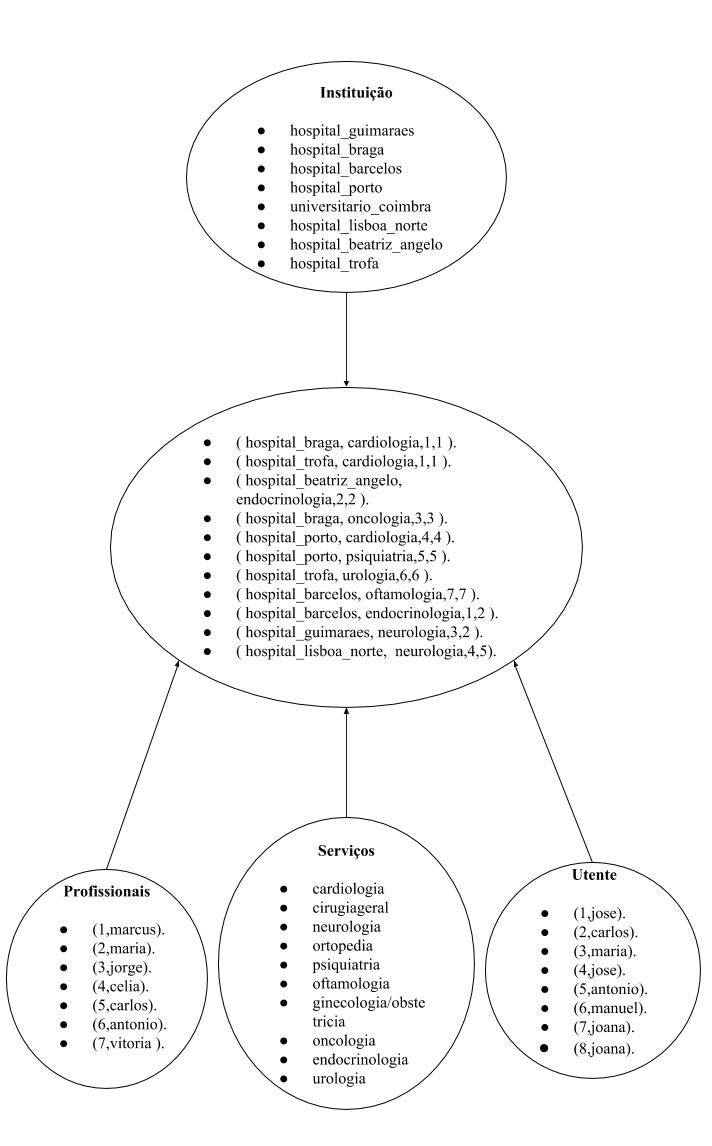
\includegraphics[scale=0.18]{esquema.jpg}
	\caption{Esquema da base de conhecimento }
	\label{p3:fig:esquema1}
\end{figure}
\newpage


\section{Funcionalidades Básicas}
\label{p3:funcbasic}

Após a apresentação da base de conhecimento do exercício torna-se possivel desenvolver alguns teoremas que consigam responder aos desafios apresentados. Desta forma, apresentaremos e explicaremos a forma como resolvemos cada um dos desafios e quais os resultados obtidos pelas soluções por nós apresentadas. 

\subsection{Identificar os serviços existentes numa instituição}
Pretende-se que seja possivel apresentar todos os serviços existentes numa determinada instituição de saúde. Para tal basta procurar todos os serviços (\textit{findall}) que estejam ligados à instituição pretendida através do axioma \textit{servicoInst(Inst,Serv)}, este que nos devolve uma lista com todos os serviços existentes numa instituição.  
Segue de seguida o axioma implementado: 
\begin{verbatim}
servicoInst(Inst,Serv):-
findall(K,ins_serv_uten_profi(Inst,K,_,_),Serv).      

servicoInst(Inst,[Serv|K]):- 
ins_serv_uten_profi(Inst,Serv,_,_),
servicoInst(Inst,K).

servicoInst(Inst,[Serv]):- 
ins_serv_uten_profi(Inst,Serv,_,_).
\end{verbatim}

Mostramos de seguida o output obtido do programa para este axioma: 

\begin{figure}[<+htpb+>]
	\centering
	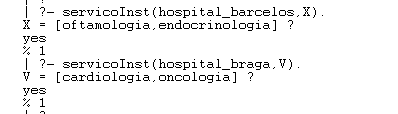
\includegraphics[scale=0.9]{answer1.png}
	\caption{Exemplo de output do axioma servicoInst}
	\label{p3:fig:output1}
\end{figure}

\subsection{Identificar os utentes de uma instituição}
Para identificar todos os utentes de uma instituição, o método será semelhante ao anterior, pois é necessário selecionar os utentes que pertencem a determinada instituição. Usamos assim o axioma \textit{utentesInst(Inst,Uten)}, que permite encontrar todos os utentes de uma dada instituição, mostramos de seguida o axioma implementado para este desafio: 

\begin{verbatim}
utentesInst(Inst,Uten):-
findall((K,J),(ins_serv_uten_profi(Inst,_,K,_),utente(K,J)),Uten).      

utentesInst(Inst,[(Cod,Uten)|K]):- 
ins_serv_uten_profi(Inst,_,Cod,_),
utente(Cod,Uten),
utentesInst(Inst,K).

utentesInst(Inst,[(Cod,Uten)]):-
ins_serv_uten_profi(Inst,_,Cod,_),
utente(Cod,Uten).
\end{verbatim}

O output produzido pela execução do axioma é:
\begin{figure}[<+htpb+>]
	\centering
	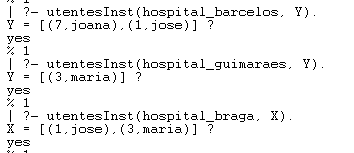
\includegraphics[scale=0.9]{answer2.png}
	\caption{Exemplo da execução do axioma utentesInst}
	\label{p3:fig:output2}
\end{figure}


\subsection{Identificar os utentes de um determinado serviço}
Mais uma vez a forma de identificar os utentes de determinado serviço é semelhante às anteriores em que usámos a funcionalidade \textit{findall} que nos devolve uma lista com os utentes, neste caso o código de utente e o respetivo nome. 

\begin{Verbatim}
servUtente(Serv,Ute):-
findall((K,J),(ins_serv_uten_profi(_,Serv,K,_),utente(K,J)),Ute).
\end{Verbatim}

Nesta cláusula é fornecida uma lista de utentes, ou penas um utente na lista e é verificado se pertencem ou pertence ao serviço pretendido: 
\begin{Verbatim}
servUtente(Serv,[(Cod,Uten)|K]):- ins_serv_uten_profi(_,Serv,Cod,_),
utente(Cod,Uten), 
servUtente(Serv,K).

servUtente(Serv,[(Cod,Uten)]):- ins_serv_uten_profi(_,Serv,Cod,_),
utente(Cod,Uten).
\end{Verbatim}


Mostrámos de seguida o output da execução do axioma: 

\begin{figure}[<+htpb+>]
	\centering
	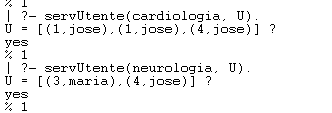
\includegraphics[scale=0.9]{answer3.png}
	\caption{Exemplo da execução do axioma servUtente}
	\label{p3:fig:output3}
\end{figure}

\subsection{Identificar os utentes de um determinado serviço numa instituição}
Para a identificação dos utentes que estão num determinado serviço numa certa instituição de saúde, implementamos o axioma \textit{utenServInst(Serv,Inst,Uten)}, este que procura o serviço e a intituição e nos devolve uma lista com os utentes. 
\begin{verbatim}
utenServInst(Serv,Inst,Uten):- 
findall((K,J),(ins_serv_uten_profi(Inst,Serv,K,_),utente(K,J)),Uten). 

utenServInst(Serv,Inst,[(Cod,Uten)|K]):-
utente(Cod,Uten),
ins_serv_uten_profi(Inst,Serv,Cod,_),
utenServInst(Serv,Inst,K).

utenServInst(Serv,Inst,[(Cod,Uten)]):-
ins_serv_uten_profi(Inst,Serv,Cod,_),
utente(Cod,Uten).
\end{verbatim}

\begin{figure}[<+htpb+>]
	\centering
	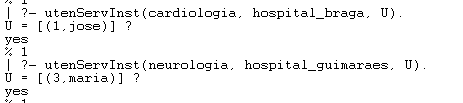
\includegraphics[scale=0.9]{answer4.png}
	\caption{Exemplo da execução do axioma utenServInst}
	\label{p3:fig:output4}
\end{figure}


\subsection{Identificar as instituições onde seja prestado um dado serviço ou conjunto de serviços}
A implementação deste axioma é semelhante aos anteriores, pois é necessário relacionar o serviço ou vários serviços à respetiva instituição. Para tal implementamos o axioma \textbf{instServico: ([Serviço],[Instituição])}, que recorre ao \textbf{servicoInst} para garantir que o serviço está na instituição e também elimina os nomes dos serviços que apareçam repetidos. 


\begin{verbatim}
 instServicos([Serv|K],I):-    
 findall(H,servicoInst(H,[Serv|K]),L),
 eliminarRepetidos(L,I).
 
 inst_Servico(S,[I|K]):- servicoInst(I,[S]),
 inst_Servico(S,K).  
 
 inst_Servico(S,[I]):- servicoInst(I,[S]).
 
 instServicos([S|T],[I|K]):-
 inst_Servico(S,[I|K]),
 instServicos(T,[I|K]).
 
 instServicos([S],[I|K]):-inst_Servico(S,[I|K]).
 
 instServicos([S],[I]):-inst_Servico(S,[I]).
\end{verbatim}

De seguida mostramos o output obtido: 

\begin{figure}[<+htpb+>]
	\centering
	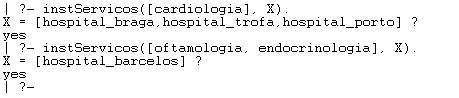
\includegraphics[scale=0.9]{answer5.png}
	\caption{Exemplo da execução do axioma instServicos}
	\label{p3:fig:output5}
\end{figure}

\subsection{Identificar os serviços que não se podem encontrar numa instituição}
Neste desafio é necessário saber quais os serviços exitentes, depois saber quais os serviços que fazem parte de uma instituição. No final subtraimos o total de serviços aos existentes em cada instituição e devolve assim os serviços que não existem em determinada instituição. Foi implementado o axioma \textbf{difList} para subtrair todos o serviços existentes aos existentes em cada instituição. 

\begin{verbatim}
todosServicos(L):-
findall(S,servico(S),L).

servicosForaInst(Ins,Serv,todos):-todosServicos(P), 
servicoInst(Ins,K),
difList(P,K,Serv).

servicosForaInst(Ins,[Serv|K]):-nao(servicoInst(Ins,[Serv|K])).
\end{verbatim}

Mostramos de seguida um exemplo da execução do programa: 

\begin{figure}[<+htpb+>]
	\centering
	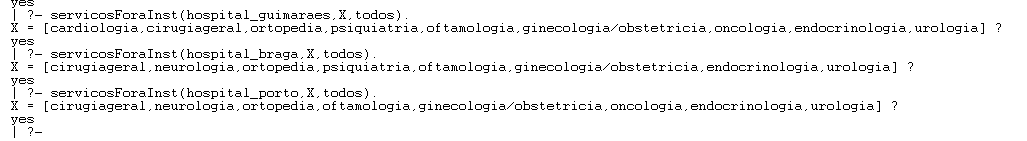
\includegraphics[scale=0.6]{answer6.png}
	\caption{Exemplo da execução do axioma servicosForaInst}
	\label{p3:fig:output6}
\end{figure}

\subsection{Determinar as instituições onde um profissional presta serviço }
Para este desafio foi necessário descobrir quais as instituições onde determinado profissional presta serviço. Para tal usamos o método de procurar todas as intituições que satisfazem o objetivo de ser um profissional que presta serviço numa determinada instituição. 
\begin{verbatim}
profiServico((Cod,Prof),Inst):- 
findall(K,(ins_serv_uten_profi(K,_,_,Cod),profissional(Cod,Prof)),Inst).

profiServico((Cod,Prof),[Inst|K]):-ins_serv_uten_profi(Inst,_,_,Cod),
profissional(Cod,Prof),
profiServico((Cod,Prof),K).

profiServico((Cod,Prof),[Inst]):-ins_serv_uten_profi(Inst,_,_,Cod),
profissional(Cod,Prof).
\end{verbatim}
Mostramos de seguida um exemplo de execução do axioma: 

\begin{figure}[<+htpb+>]
	\centering
	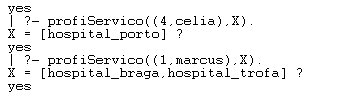
\includegraphics[scale=0.9]{answer7.png}
	\caption{Exemplo da execução do axioma profiServico}
	\label{p3:fig:output7}
\end{figure}

\subsection{Determinar todas as instituições(ou serviços ou profissionais) a quem o utente já recorreu}

Este desafio foi realizado por partes, pois é necessário saber quais as intituições todas a que um utente já recorreu, começamos por criar o axioma \textbf{instSerProf((Cod,Uten),Inst,ints)}, em que quando se dá um utente devolve uma lista de instituições onde esse utente já frequentou. 

De seguida implementamos o axioma \textbf{instSerProf((CodU,Uten),Serv,serv)}, que permite saber quais os serviços que um utente já frequentou. 
Por fim construímos o axioma \textbf{instSerProf((CodU,Uten),Prof,prof)}, que nos devolve uma lista com os profissionais a quem determinado utente recorreu. Todos estes axiomas estão a eliminar informação repetida. 

\begin{verbatim}
instSerProf((Cod,Uten),Inst,ints):-
 findall(K,(ins_serv_uten_profi(K,_,Cod,_),utente(Cod,Uten)),L),
eliminarRepetidos(L,Inst).

instSerProf((CodU,Uten),Serv,serv):-
findall(K,(ins_serv_uten_profi(_,K,CodU,_),utente(CodU,Uten)),L),
eliminarRepetidos(L,Serv).

instSerProf((CodU,Uten),Prof,prof):-
findall((K,Nome),(ins_serv_uten_profi(_,_,CodU,K),utente(CodU,Uten),
profissional(K,Nome)),L),
eliminarRepetidos(L,Prof).
\end{verbatim}

Exemplificamos na imagem abaixo a execução dos axiomas acima descritos: 

\begin{figure}[<+htpb+>]
	\centering
	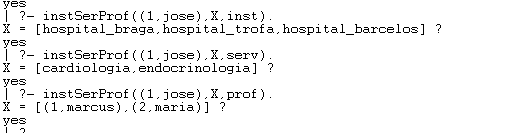
\includegraphics[scale=0.9]{answer8.png}
	\caption{Exemplo da execução do axioma instSerProf}
	\label{p3:fig:output8}
\end{figure}


\subsection{Registar utentes, profissionais, serviços ou instituições}
Para possibilitar a inserção de conhecimento na base implementamos o teorema \textbf{inserirConhecimento}, este teorema que necessita de verificar os invariantes definidos por nós, pois não podiamos deixar que informação repetida fosse adicionada à base de conhecimento. Fica de seguida um exerto de como implementamos as inserções na base de conhecimento: 

\begin{Verbatim}
adicionarUtentes(Codigo,Utente):- 
inserirConhecimento(utente(Codigo,Utente)).

adicionarServico(Servico):- 
inserirConhecimento(servico(Servico)).

adicionarProfissional(Codigo,Profissional):-
 inserirConhecimento(profissional(Codigo,Profissional)).

adicionarInstituicao(Nome):- 
inserirConhecimento(instituicao(Nome)).
\end{Verbatim}

Criamos vários invariantes para garantir que não é inserido conhecimento repetido no sistema. 

O primeiro invariante criado não permite que seja introduzido de novo um utente já existente. Foi criado outro invariante muito semelhante a este mas para a inserção de um novo profissional. No código em baixo pode-se verificar a implementação do invariante que não permite a inserção de utentes repetidos: 


\begin{Verbatim}
+utente(Codigo,Uten) :: (solucoes( (Codigo,Uten),
 utente(Codigo,Uten), S),comprimento(S,N),N==1).
\end{Verbatim}

O segundo invariante não permite introduzir um código de utente já existente, assim como também implementamos para o profissional o mesmo invariante: 
\begin{Verbatim}
+utente(Codigo,_) :: (solucoes( Uten, utente(Codigo,Uten), S),
comprimento(S,N),N==1).
\end{Verbatim}

No terceiro invariante não permitimos que se introduzisse o mesmo nome a uma intituição, partindo do facto que não existem instituições com o mesmo nome. 

\begin{Verbatim}
+instituicao(Nome) :: (solucoes( Nome, instituicao(Nome), S),
comprimento(S,N),N==1). 
\end{Verbatim}
No quarto inavariante não permitimos que se introdizem o mesmo nome para um serviço. 

\begin{Verbatim}
+servico(Nome) :: (solucoes( Nome, servico(Nome), S),
comprimento(S,N),N==1). 
\end{Verbatim}

Mostramos de seguida a execução dos teoremas e a respetiva listagem com os dados inseridos na base de conhecimento. 

\begin{figure}[<+htpb+>]
	\centering
	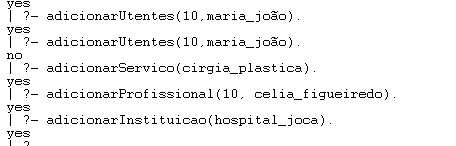
\includegraphics[scale=0.9]{answer9.png}
	\caption{Exemplo da execução do axioma adicionar utente ou serviço com a respetiva listagem de dados}
	\label{p3:fig:output9}
\end{figure}

\subsection{Remover utente (profissionais, serviços, instituições) dos registos}

Para possibilitar a remoção de conhecimento foi necessário criar o predicado \textbf{remover}, este predicado também necessita de verificar invariantes criados por nós. Mostramos de seguida o exercerto dos predicados de remoção :

\begin{Verbatim}
removerUtentes(Codigo,Utente):- remover(utente(Codigo,Utente)).

removerServico(Servico):- remover(servico(Servico)).

removerProfissional(Codigo,Profissional):-
 remover(profissional(Codigo,Profissional)).

removerInstituicao(Nome):- remover(instituicao(Nome)).
\end{Verbatim}

O primeiro invariante criado não permite que seja removido um utente enquanto estiver a ser consultado: 

\begin{Verbatim}
-utente(Codigo,Nome) :: (nao(ins_serv_uten_profi(_,_,Codigo,_)),
nao(utente(Codigo,Nome))).
\end{Verbatim}

O segundo invariante não permite remover um profissional enquanto este estiver num serviço ou instituição. 

\begin{Verbatim}
-profissional(Codigo,Nome) :: (nao(ins_serv_uten_profi(_,_,_,Codigo)),
nao(profissional(Codigo,Nome))).
\end{Verbatim}

O terceiro invariante não permite  que seja removido um servico com profissionais a trabalhar nele ou utentes a usá-lo, ou estar na instituicao

\begin{Verbatim}
-servico(Nome) :: (nao(ins_serv_uten_profi(_,Nome,_,_))).
\end{Verbatim}

O quarto invariante não permite remover uma instituicao com profissionais, utentes, ou servicos
\begin{Verbatim}
-instituicao(Nome) :: (nao(ins_serv_uten_profi(Nome,_,_,_))).
\end{Verbatim}

Mostramos de seguida um exemplo de remoção de conhecimento: 

\begin{figure}[<+htpb+>]
	\centering
	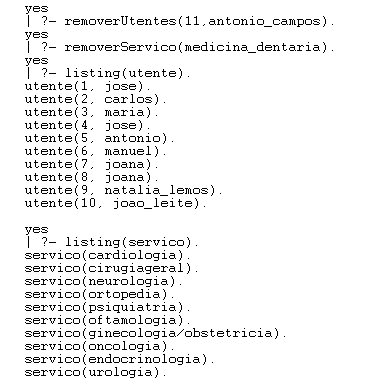
\includegraphics[scale=0.9]{answer10.png}
	\caption{Exemplo da execução do axioma profiServico}
	\label{p3:fig:output10}
\end{figure}

\newpage

\subsection{Funcionalidades Extra}

Após a conclusão das funcionalidades básicas exigidas e de forma a enriquecer o nosso exercício decidimos implementar funcionalidades extra. 
Assim sendo, passaremos a explicar estas novas funcionalidades, que se baseiam na contagem de entidades no sistema. 

\subsubsection{Contagem de utentes, serviços, profissionais e instituições}

Para a inserção desta funcionalidade foi necessária a criação de um predicado que permitisse calcular o comprimento de uma lista, para tal implementou-se o predicado \textbf{comprimento}:
\begin{Verbatim}
comprimento([], 0).
comprimento([_|T], R) :-
comprimento(T, X),
R is 1+X.
\end{Verbatim}

Para a contagem das caracteristicas pretendidas em cada caso o método utilizado foi semelhante, aplicámos o predicado \textbf{comprimento} aos elementos pretendidos, como segue no exemplo de contar o número de serviços existentes em determinada instituição de saúde: 

\begin{Verbatim}
numero_Servico(Inst,N):- servicoInst(Inst,K),comprimento(K,Contador), 
N is Contador.
\end{Verbatim}

Um outro exemplo é o da contagem dos profissionais existentes em determinada instituição de saúde em que se utilizou o \textbf{findall}. Este mecanismo serve para encontrar todos os profissionais em determinada instituição, com o objetivo de obter o comprimento da lista (contador). O resultado será unificado,  \textbf{N} passará a assumir esse resultado, como se pode verificar na implementação deste predicado abaixo:  

\begin{Verbatim}
numero_Profissionais(Inst,N):-
 findall(Prof,ins_serv_uten_profi(Inst,_,_,Prof),L),
comprimento(L,Contador), 
N is Contador.
\end{Verbatim}

\subsubsection{Adicionar e remover conhecimento}

Criou-se também um mecanismo que permite a inserção de uma instituição, um serviço um utente e um profissional. 

\begin{Verbatim}
adicionarInstServico(Inst,Serv,CodUten,CodProf):- 
inserirConhecimento(ins_serv_uten_profi
(Inst,Serv,CodUten,CodProf)).
\end{Verbatim}

Por outro lado criamos também um mecanismo para a remoção destes conhecimentos :
\begin{Verbatim}
removerInstServico(Inst,Serv,CodUten,CodProf):- 
remover(ins_serv_uten_profi(Inst,Serv,CodUten,CodProf)).
\end{Verbatim}

\subsubsection{Invariantes Criados}
Criámos um inavariante que não deixa inserir  um hospital, servico, utente ou profissional que nao exista:

\begin{Verbatim}
+ins_serv_uten_profi(Inst,Serv,CodUten,CodProf) :: 
(solucoes((Inst,Serv,CodUten,CodProf),
(utente(CodUten,_),profissional(CodProf,_),
instituicao(Inst),servico(Serv)),K), comprimento(K,N),N==1).
\end{Verbatim}

Implementámos também um inavriante que não permite a inserção de conhecimento repetido: 

\begin{Verbatim}
+ins_serv_uten_profi(Inst,Serv,CodUten,CodProf) ::
 (solucoes((Inst,Serv,CodUten,CodProf),
(ins_serv_uten_profi(Inst,Serv,CodUten,CodProf)),K),
 comprimento(K,N),N==1).
\end{Verbatim}



Mostramos de seguida todos os exemplos de execução da nossas funcionalidades extra: 
\begin{figure}[<+htpb+>]
	\centering
	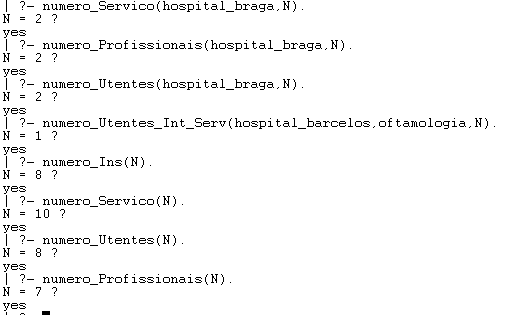
\includegraphics[scale=0.9]{extras.png}
	\caption{Exemplo da execução dos extras do exercício}
	\label{p3:fig:output10}
\end{figure}


